

\section{Nem-transzverzális metszés: Grazing [Zsiros Ádám, impakt oscillátor - nincs kész]}

Tekintsük az alábbi rendszert:
\begin{equation}
\dot{x}=F(x), \quad \text{ahol } x\in S^+=\left\{x\in\mathcal{D}\subset\mathbb{R}^n: H(x)>0\right\},
\end{equation}
amely a 
\begin{equation}
\sum:=\left\{x\in\mathcal{D}: H(x)=0\right\}
\end{equation}
felületen ütközik az
\begin{equation}
x^+=R(x^-):=x^-+W(x^-)v(x^-)
\end{equation}
leképezés által kijelölt módon. $H(x)$ a kapcsolóvonal egyenlete, $x^+$ az ütközés utáni állapotváltozó, $x^-$ pedig az ütközés előtti állapotváltozó. Az ütközés pillanatában a kapcsolófelületre merőleges sebességet és gyorsulást a 
\begin{equation}
v(x)=H_xF(x), 
\end{equation} 
a gyorsulást pedig 
\begin{equation}
 a(x)=(H_{xx}+H_xF_x)F(x)
\end{equation} 
összefüggés segítségével számíthatók ki.

\subsection{1DoF impakt oszcillátor}


Az 1 DoF impakt oszcillátor dimenziótlan egyenlete az alábbi:
\begin{equation}
u''(t)+2\zeta u'(t)+u(t)=w(t),\qquad u(t)>\sigma,\qquad \zeta>0.
\end{equation}
A $t=t_0$ (ütközéskori) időpillanatban az alábbi leképezés valósul meg:
\begin{equation}
f(u^-,v^-):=(u^+,v^+),
\end{equation}
ahol közvetlenül az ütközés előtti pozíció és sebesség
\begin{equation}
u^-=u(t_0),
\end{equation}
\begin{equation}
v^-=v(t_0)=\left.\frac{\mathrm{d}u}{\mathrm{d}t}\right|_{t=t_0},
\end{equation}
továbbá a közvetlenül az ütközés utáni pozíció és sebesség felírható az alábbi módon:
\begin{equation}
u^+=u^-,
\end{equation}
\begin{equation}
v^+=-rv^-, \quad 0\le r\le 1.
\end{equation}
Megjegyzés: $1-r^2$ meghatározza az ütközés során elnyelt mozgási energiaarányt. $r$ a különböző anyagok tulajdonságaitól függ, $r=0.95$ az acélrúd esetének felel meg, $r=1$ a tökéletesen rugalmas és $r=0$ a tökéletesen rugalmatlan ütközésnek felel meg. Az általunk vizsgált esetben $w(t)=\cos(\omega t)$ a periodikus gerjesztés $\frac{2\pi}{\omega}$ periódussal:
\begin{equation}
u''(t)+2\zeta u'(t)+u(t)=\cos(\omega t),\qquad u>\sigma.
\end{equation}
Az 1DoF impakt oszcillátor átírható az alábbi három-dimenziós autonóm rendszerré:
\begin{equation}
\begin{split}
\frac{\mathrm{d}u}{\mathrm{d}t}&=v,\\
\frac{\mathrm{d}v}{\mathrm{d}t}&=-u-2\zeta v+w(s),\\
\frac{\mathrm{d}s}{\mathrm{d}t}&=1,
\end{split}\qquad \qquad \text{ha } u>\sigma,
\end{equation}
azaz az alábbi lineáris differenciálegyenlet írja le a rendszert:
\begin{equation}
\dot{x}=F(x),
\end{equation}
ahol
\begin{equation}\label{eq:xFx}
x=\begin{pmatrix}
u\\ v\\ s
\end{pmatrix},\qquad
F(x)=\begin{pmatrix}
v\\
-u-2\zeta v+w(s)\\
1
\end{pmatrix}.
\end{equation}
A kapcsolóvonal egyenlete
\begin{equation}
H(x)=u-\sigma,
\end{equation}
gradiense pedig

\begin{equation}\label{eq:hx}
H_x=\begin{pmatrix}
1\\
0\\
0
\end{pmatrix}.
\end{equation}
A leképezés a kapcsolóvonalon:

\begin{equation}
x \rightarrow R(x)=\begin{pmatrix}
u\\
-r v\\
s,
\end{pmatrix}
\end{equation}
azaz a leképezés gradiense

\begin{equation}\label{eq:Rx}
R_x(x)=\begin{pmatrix}
1 & 0 & 0\\
0 & -r & 0\\
0 & 0 & 1
\end{pmatrix}.
\end{equation}
A sebesség, illetve a gyorsulás az alábbi módon írható le:
\begin{equation}
v(x)=v,
\end{equation}
\begin{equation}
a(x)=-u-2\zeta v+w(s),
\end{equation}
%
így kapcsolóvonalra történő becsapódási sebesség:

\begin{equation}
H_x(x^-) F(x^-) = v^-,
\end{equation}
Újra megemlítjük a \eqref{eq:Qxmatrix} egyenletre levezetett korrekciós mátrixot:

\begin{equation}\label{eq:Qxmatrix2}
Q_x(x^-)=R_x(x^-)+\frac{F(R(x^-))-R_x(x^-)F(x^-)}{H_x(x^-)F(x^-)}H_x(x^-)\,,
\end{equation}
ahol $x^-$ legyen egy periodikus pálya ütközési pontja. Felhasználva, hogy 
\begin{equation}
x^+=R(x^-),
\end{equation}
azaz az ütközés utáni állapot felírható az ütközés előtti állapot és leképezés segítségével. \eqref{eq:xFx}, \eqref{eq:hx}, \eqref{eq:Rx} egyenletek felhasználásával:

\begin{equation}
\begin{split}
Q_x(x^-)=\begin{pmatrix}
1 & 0 & 0\\
0 & -r & 0\\
0 & 0 & 1
\end{pmatrix}+\frac{\left(F(x^+)-R_x(x^-)F(x^-)\right)H_x}{v^-}=\\
=\begin{pmatrix}
1 & 0 & 0\\
0 & -r & 0\\
0 & 0 & 1
\end{pmatrix}+\frac{1}{v^-}\left(\begin{pmatrix}
v^+-v^-\\
a^-(-ra^-)\\
t^--t^-
\end{pmatrix} \right)H_x=\begin{pmatrix}
r & 0 & 0\\
\frac{a^++ra^-}{v^-} & -r & 0\\
0 & 0 & 1
\end{pmatrix}.
\end{split}
\end{equation}

A numerikus megoldást a fázistérben különböző gerjesztési frekvenciák esetére a \ref{fig:phase}. ábra szemlélteti, a numerikusan meghatározott elmozdulásfüggvényeket szintén különböző gerjesztési frekvenciák esetére a \ref{fig:ut}. ábra szemlélteti. A \ref{fig:phase}--\ref{fig:ut}. ábrák elkészítése az alábbi fejezetben található \textit{Matlab}-kóddal valósítható meg: \ref{ap:codes1}. fejezet.


\begin{figure}[h!]
\centering
\begin{subfigure}[b]{0.31\linewidth}
         \centering
         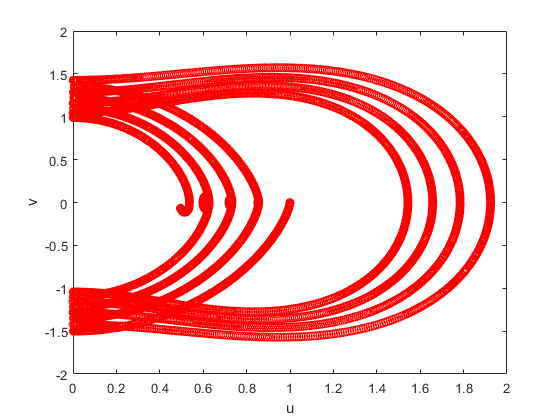
\includegraphics[width=1\linewidth]{graphics/uv_w3_r095_omega0_ksi0.png}
         \caption{$\omega=3$}
         \label{fig:w3000}
     \end{subfigure}
     \begin{subfigure}[b]{0.31\linewidth}
         \centering
         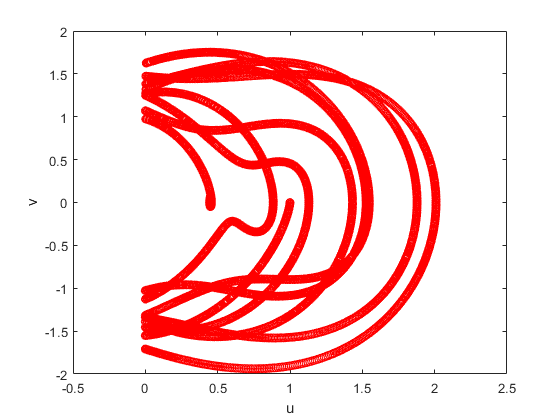
\includegraphics[width=1\linewidth]{graphics/uv_w276_r095_omega0_ksi0.png}
         \caption{$\omega=2,76$}
         \label{fig:w276}
     \end{subfigure}
     \begin{subfigure}[b]{0.31\linewidth}
         \centering
         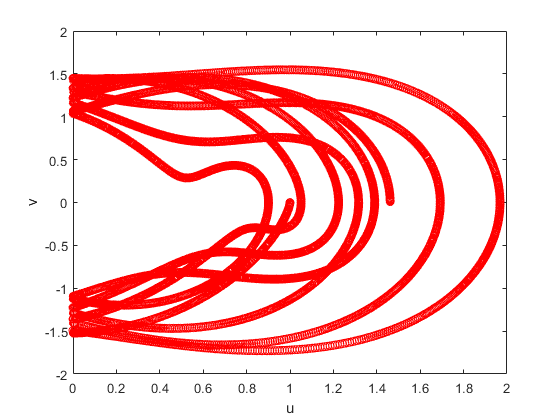
\includegraphics[width=1\linewidth]{graphics/uv_w29_r095_omega0_ksi0.png}
         \caption{$\omega=2,9$}
         \label{fig:w290}
     \end{subfigure}
     \caption{Az 1DoF impakt oszcillátor fázisportréi $\sigma =0$, $r=0.95$, $\zeta =0$ esetre különböző gerjesztési frekvenciák esetén}\label{fig:phase}
\end{figure}

\begin{figure}[h!]
\centering
\begin{subfigure}[b]{0.31\linewidth}
         \centering
         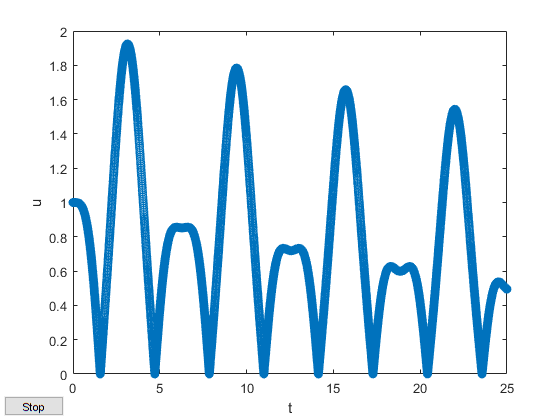
\includegraphics[width=1\linewidth]{graphics/ut_w3_r095_omega0_ksi0.png}
         \caption{$\omega=3$}
         \label{fig:w3000_1}
     \end{subfigure}
     \begin{subfigure}[b]{0.31\linewidth}
         \centering
         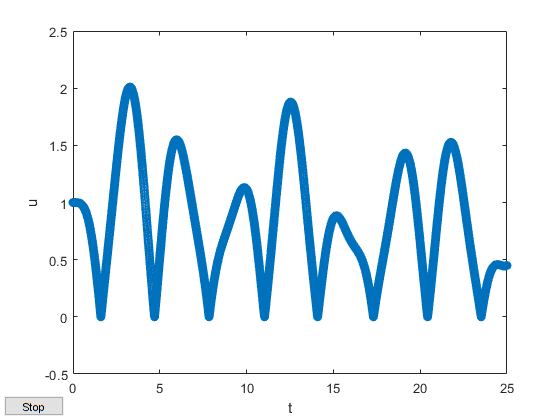
\includegraphics[width=1\linewidth]{graphics/ut_w276_r095_omega0_ksi0.png}
         \caption{$\omega=2,76$}
         \label{fig:w276_1}
     \end{subfigure}
     \begin{subfigure}[b]{0.31\linewidth}
         \centering
         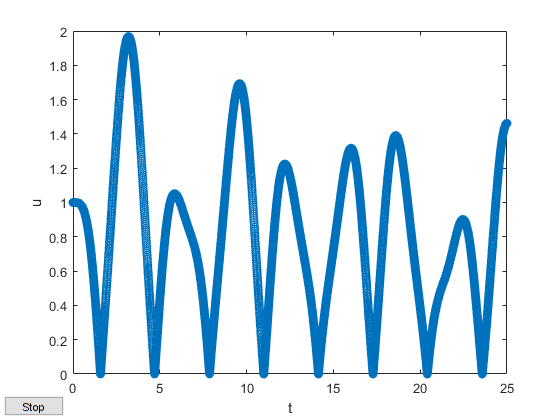
\includegraphics[width=1\linewidth]{graphics/ut_w29_r095_omega0_ksi0.png}
         \caption{$\omega=2,9$}
         \label{fig:w290_1}
     \end{subfigure}
     \caption{Az 1DoF impakt oszcillátor rezgése $\sigma=0$, $r=0.95$, $\zeta=0$ esetre különböző gerjesztési frekvenciák esetén}\label{fig:ut}
\end{figure}

Az ütközés és a leképezés pontjainak számítása az alábbi módon történik:
1. Kiszámítjuk a $0<t<T$ folytonos szakasz monodrómiai mátrixát:
\begin{equation}
x^*=M x_0
\end{equation}

2. Kiszámítjuk a korrekciós mátrixot (saltation matrix)

\begin{equation}
x_0=Q_x x^*
\end{equation}

3. A teljes monodrómia mátrix:
\begin{equation}
x_0^{n+1}=Q_x M x_0^n
\end{equation}

\subsection{Ütközés nélküli eset -- monodrómia mátrix}
Tegyük fel, hogy $\left(u(t),v(t)=\frac{\mathrm{d}u}{\mathrm{d}t}\right)$ megoldása a 
\begin{equation}
u''(t)+2\zeta u'(t)+u=w(t)
\end{equation}
egyenletnek. Tekintsük az alábbi perturbált megoldást: $\left(u(t)+\delta u(t),v(t)+\delta v(t)\right)$. A $\delta u$ függvény kielégíti az alábbi variációs egyenletet
\begin{equation}
\delta u''(t)+2\zeta \delta u'(t)+\delta u=0,\qquad \left(\delta u(t_0),\delta v(t_0) \right)=\left(\delta u_0,\delta v_0 \right),
\end{equation}
azaz
\begin{equation}
\frac{\mathrm{d}}{\mathrm{d}t}\begin{pmatrix}
\delta u\\ \delta v
\end{pmatrix}=L\begin{pmatrix}
\delta u\\ \delta v
\end{pmatrix}:=\begin{pmatrix}
0 & 1 \\
-1 & -2\zeta
\end{pmatrix}\begin{pmatrix}
\delta u\\ \delta v
\end{pmatrix}.
\end{equation}
Így felírható az egy $(T)$ periódusra vonatkozó állapotvektor variációja:
\begin{equation}
\begin{pmatrix}
\delta u_T\\ \delta v_T
\end{pmatrix}:=
\begin{pmatrix}
\delta u(t_0+T)\\
\delta v(t_0+T)
\end{pmatrix}
=\mathrm{e}^{LT}\begin{pmatrix}
\delta u(t_0)\\ \delta v(t_0)
\end{pmatrix}.
\end{equation}
Így az egy periódusra vonatkozó leképezés (monódrómia) mátrixa
\begin{equation}\label{eq:Nt}
N_T=\mathrm{e}^{LT}=\mathrm{e}^{-\zeta T}\begin{pmatrix}
C_T & S_T\\
-\zeta C_T-\omega_0S_T & \omega_0C_T-\zeta S_T
\end{pmatrix},
\end{equation}
ahol 
\begin{equation}
\omega_0=\sqrt{1-\zeta^2},
\end{equation}
\begin{equation}
C_T=\cos(\omega_0T),
\end{equation}
\begin{equation}
S_T=\sin(\omega_0T).
\end{equation}
Érdemes megemlíteni, hogy 
\begin{equation}
\det\left(N_T \right)=\mathrm{e}^{-2\zeta T},
\end{equation}
azaz a rendszer disszipatív, ha $\zeta>0$.

\subsection{Ütközéses eset -- korrekciós mátrix}

Tegyük fel, hogy a $T$ időintervallumban ütközés történik a $t=t_0+t_I$ időpillanatban. Az ütközés előtti sebesség $v_I<0$, az ütközés előtti gyorsulás $a_I^-$, az ütközés utáni gyorsulás pedig $a_I^+$. A mozgás dinamikáját módosítja az ütközés, ennek leírásához pedig a $Q_x$ mátrix kerül kiszámításra (\eqref{eq:Qxmatrix2} egyenlet). Így a $T$ periódusra vonatkozó állapotvektor-variáció az alábbi módon írható le:
\begin{equation}
\begin{pmatrix}
\delta u_T\\ \delta v_T
\end{pmatrix}:=
\begin{pmatrix}
\delta u(t_0+T)\\
\delta v(t_0+T)
\end{pmatrix}
=\tilde{N}_T\begin{pmatrix}
\delta u_0\\ \delta v_0
\end{pmatrix},
\end{equation}
ahol $\tilde{N}_T$ (\eqref{eq:Nt} egyenlet felhasználásával) az alábbi módon számolható:
\begin{equation}
\tilde{N}_T=N_{T-t_I}Q_xN_{t_I}.
\end{equation}
Jelen esetben $\tilde{N}_T$ determinánsa
\begin{equation}
\det\left( \tilde{N}_T\right)=\mathrm{e}^{-2\zeta T}r^2.
\end{equation}
Általánosítva ($m$ ütközés történik a $T$ periódus alatt):
\begin{equation}
\det\left(\tilde{N}_T \right)=\mathrm{e}^{-2\zeta T}r^{2m}.
\end{equation}
Megfigyelhető, hogy a rendszer disszipatív, ha $r<1$, feltéve, ha $\zeta \leq 0$.

\subsection{Linearizálás}

Tegyük fel, hogy az $u(t)$ mozgás periodikus az alábbi feltételekkel: $v(t_0)=v(t_0+T)=0$, $a_0:=a(t_0)\neq 0$. Kiszámításra kerül a $P_N$ leképezés linearizálása, ami a $\Pi_N=\left\{(u,t):v=0\right\}$ felületről képez le önmagára. Ehhez tekintsük a kezdeti feltételek kis perturbálását és vizsgáljuk a rendszer viselkedésének változását $t_0+\delta t_0$ kezdeti időpillanattól $t_0+T+\delta T$ időpillanatig. A feltételek:
\begin{equation}
u(t_0+\delta t_0)=u(t_0)+\delta u_0,
\end{equation}
\begin{equation}
v(t_0+\delta t_0)=0;
\end{equation}
\begin{equation}
u(t_0+T+\delta T)=u(t_0+T)+\delta u_T,
\end{equation}
\begin{equation}
v(t_0+T+\delta T)=0.
\end{equation}
Kis $\delta t_0$ és $\delta u_0$ értékekre a $P_T$ evolúciós leképezés 
\section{Grazing}

Amennyiben egy $x^*$ pontban igazak az alábbiak
\begin{equation}
H(x^*)=0,
\end{equation}
\begin{equation}
a(x^*)>0,
\end{equation}
\begin{equation}
H_x(x^*) F(x^*) = 0,
\end{equation}
akkor \emph{reguláris} grazing pontról beszélünk.

Belátható, hogy a grazing-bifurkáció környezetében a $p(t)$ periodikus pálya körüli dinamikát az alábbi linearizált Poincaré-leképezés  írja le (ld. könyv 193 -- 198.o. ill. 6. fejezet)

% $x\rightarrow f(x,\mu), \quad x \in \mathbb{R}^{n}, \quad \mu \in \mathbb{R}^n, \; $ ahol
\begin{equation}\label{eq:nordmark}
P_N(x,\mu)=\begin{cases}
Nx+M\mu+Ey, \quad &\text{ha} \; H(x,\mu)<0\\
Nx+M\mu, &\text{ha} \; H(x,\mu)>0
\end{cases}
\end{equation}

\noindent ahol $N=\partial_x \tilde{P}_N(x^*,\mu^*)$ és $M=\partial_\mu \tilde{P}_N(x^*,\mu^*)$ és 

\begin{equation}
y=\sqrt{-C^TNx-(C^T M+D)\mu}+O(x,\mu)=\sqrt{-H(x,\mu)}+O(x,\mu)
\end{equation}

\noindent és $E$ egy további (bonyolult) függvény és $C$ ill. $D$ a $H(x)$ linearizálása, azaz 
\begin{equation}
\left.H(x)\right|_{x^*}=C^T(\tilde{x}-x^*)+D(\tilde{\mu}-\mu^*)=C^T (Nx+M\mu)+D \mu.
\end{equation}

\noindent A \eqref{eq:nordmark} rendszert hívjuk Nordmark leképezésnek.

\section{Fixpont}

A \eqref{eq:nordmark} rendszer fixpontja

\begin{equation}
x_e=(I-N)^{-1}M \mu,
\end{equation}

\noindent és ha bevezetjük a $z=x-x_e$ új koordinátát, akkor a

\begin{equation}
z \mapsto f(z)=\begin{cases}
Nz+E\sqrt{\sigma-C^T N z}, \quad &\text{ha} \; C^T N z<\sigma\\
Nz, &\text{ha} \; C^T N z>\sigma
\end{cases}
\end{equation}

\noindent rendszert kapjuk, ahol azt, hogy $z$ képe ütközik-e vagy nem, a $H=H(x^*,\mu)+C^T N z$ előjele dönti el, ahol $\sigma=-H(x^*,\mu)$.

\subsection{A "square root" leképezés}

[ide esetleg jöhet, hogy az előző rendszerből pontosan hogyan is lesz a jelenlegi]

A fenti rendszer tovább egyszerűsíthető. Mivel egy lineáris leképezésről van szó, az iterációk viselkedését a $\nu_1$ legnagyobb sajátérték fogja megadni és formálisan elegendő a

\begin{equation}\label{eq:sr}
w \mapsto f(w)=\begin{cases}
\nu w+\sqrt{\mu-w}, \quad &\text{ha} \; w-\mu<0\\
\nu w, &\text{ha} \; w-\mu>0
\end{cases}
\end{equation}

\noindent leképezést vizsgálni. Szakaszos ,,square-root'' leképezések azon folytonos leképzések, amelyeknél a leképezés egyik szakaszán négyzetgyökös, másik szakaszán pedig lineáris a leképezés. Az \eqref{eq:sr} leképezés esetén készített square-root mapeket $\nu=0,9$ esetén különböző $\mu$ értékekre a \ref{fig:square-root}. ábra szemlélteti.


\begin{figure}[ht!]
\centering
\begin{subfigure}[b]{0.45\linewidth}
         \centering
         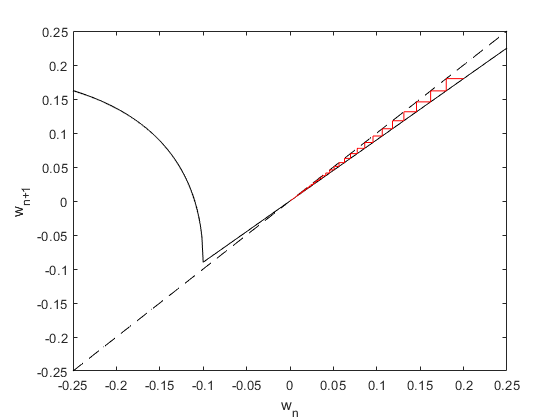
\includegraphics[width=1\linewidth]{graphics/sr_m01.png}
         \caption{$\mu=-0.1$}
         \label{fig:s_m01}
     \end{subfigure}
     \begin{subfigure}[b]{0.45\linewidth}
         \centering
         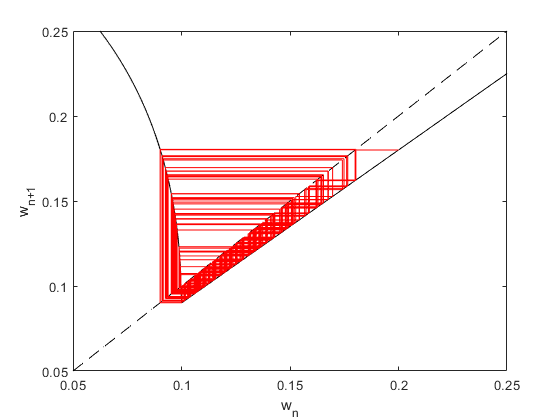
\includegraphics[width=1\linewidth]{graphics/sr_01.png}
         \caption{$\mu=0.1$}
         \label{fig:s_01}
     \end{subfigure}
     \caption{Egy dimenziós square-root map különböző $\mu$ értékekre $\nu=0,9$ esetén}\label{fig:square-root}
\end{figure}

A \ref{fig:square-root}. ábrán látható square-root leképezések esetén, ha kézzel szeretnénk elvégezni a ,,pókháló-diagram'' elkészítését, akkor az alábbi lépéseket szükséges megtennünk:
\begin{enumerate}
\item Vegyük fel a leképezés görbéjét, azaz \eqref{eq:sr} egyenletet (fekete folytonos vonal a \ref{fig:square-root}. ábrán)!
\item Vegyük fel az $x_n=x_{n+1}$ egyenest (fekete szaggatott vonal a \ref{fig:square-root}. ábrán)!
\item Vegyük fel a kezdeti feltételt az $x_n$ tengelyen!
\item Vetítsük a kezdeti feltételt az $x_n$ tengelyről a leképezés görbéjére!
\item Az így kapott $P_0(x_{n},x_{n+1})$ pont két koordinátája az $x_n$, illetve az $x_{n+1}$. Következő lépésben azt szükséges elérni, hogy a leképezés következő pontja a $P_1(x_{n+1},x_{n+2})$ pont legyen, azaz az új pont első koordinátájának az előző pont második koordinátájával kell megegyeznie. Ennek lépései: 
\begin{enumerate}
\item $P_0(x_{n},x_{n+1})$ pontból eljutunk a $\tilde{P}_0(x_{n+1},x_{n+1})$ pontba, azaz az $x_n$ tengellyel párhuzamosan rávetítjük a $P_0$ pontot az $x_n=x_{n+1}$ egyenesre.
\item A $\tilde{P}_0(x_{n+1},x_{n+1})$ pontból eljutunk az $P_1(x_{n+1},x_{n+2})$ pontba: az $\tilde{P}_0$ pont első koorinátája meg kell, hogy egyezzen a $P_1$ pont első koordinátájával, és tudjuk, hogy $P_1$ a leképezés görbéjén van, így a $\tilde{P}_0$ pontot szükséges rávetíteni a leképezés görbéjére az $x_{n+1}$ tengellyel párhuzamosan.
\end{enumerate} 
\item Ismételjük meg a folyamatot $N$-szer!
\end{enumerate}

A \ref{fig:square-root}. ábrán látható, hogy a \ref{fig:s_m01}. ábrán egy olyan paraméterkombináció került kiválasztásra, ahol $x=0$ a stabil fixpont, míg \ref{fig:s_01}. ábrán egy olyan paraméterkombináció került kiválasztásra, ahol jóval komplikáltabb viselkedése van a rendszernek. A grazing bifurkáció viselkedése a $\mu$ paraméter értékétől függ, három esetet lehetséges elkülöníteni:
\begin{enumerate}
\item Kis csillapítás, $2/3<\nu<1$: amint $\nu$ átlépi a 0-t, a rendszert kaotikus mozgás jellemzi (\ref{fig:kis_csillapitas}. ábra).
\item Közepes csillapítás, $1/4<\nu<2/3$: ,,ablakok végtelen sorozata'', amelyekben egymást váltja a stabil periodikus mozgás és a kaotikus mozgás. Az egyes ablakok között 1-gyel csökken a egyensúlyi helyek száma (\ref{fig:kozepes_csillapitas}. ábra).
\item Nagy csillapítás, $0<\nu<1/4$: ebben az esetben nincs kaotikus mozgás, de a egyensúlyi hely csökkenés az egyes ,,ablakok'' között itt is jelen van  (\ref{fig:nagy_csillapitas}. ábra).
\end{enumerate}

Az egyes eseteket a \ref{fig:bif}. ábra szemlélteti egy-egy adott $\nu$ érték esetén.

\begin{figure}[ht!]
\centering
\begin{subfigure}[b]{0.45\linewidth}
         \centering
         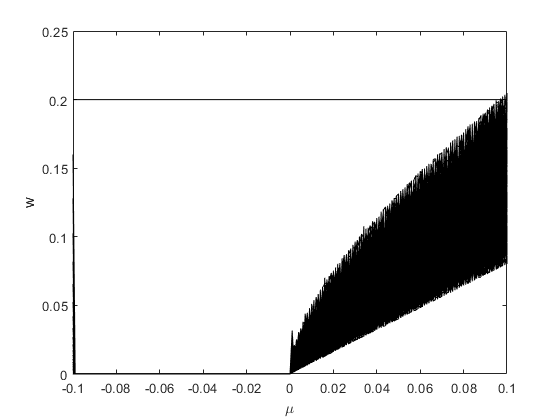
\includegraphics[width=1\linewidth]{graphics/bif_08.png}
         \caption{$\nu=0.8$}
         \label{fig:kis_csillapitas}
     \end{subfigure}
     \begin{subfigure}[b]{0.45\linewidth}
         \centering
         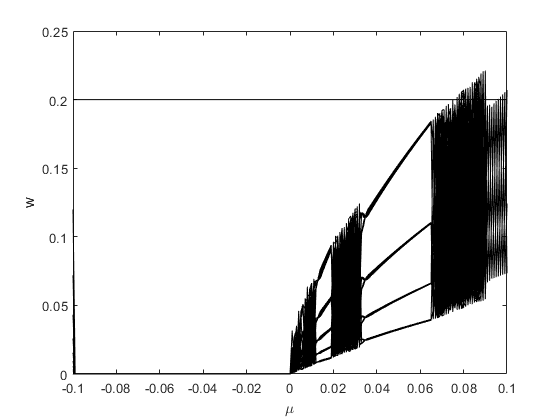
\includegraphics[width=1\linewidth]{graphics/bif_06.png}
         \caption{$\nu=0.6$}
         \label{fig:kozepes_csillapitas}
     \end{subfigure}
     \begin{subfigure}[b]{0.45\linewidth}
         \centering
         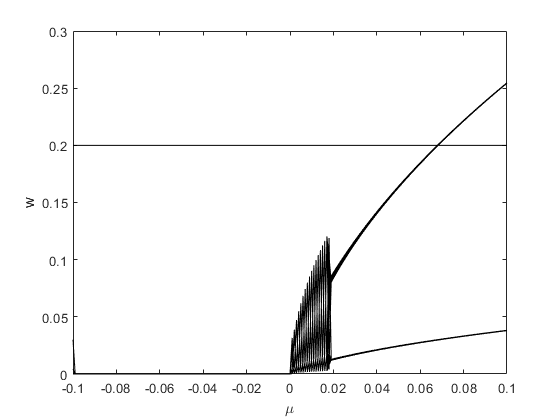
\includegraphics[width=1\linewidth]{graphics/bif_015.png}
         \caption{$\nu=0.15$}
         \label{fig:nagy_csillapitas}
     \end{subfigure}
     \caption{Bifurkációs diagram az 1D square-root mapra vonatkozóan különböző $\nu$ értékek esetén (bifurkációs paraméter: $\mu$)}\label{fig:bif}
\end{figure}

\newpage
\subsection{Kódok -- 1.}\label{ap:codes1}

\begin{lstlisting}
clear all
close all
clc

global zeta
global w
global r
global sigma

zeta=0;
w=3;
r=0.8;
sigma = 0;

tMon=2*pi/w;
tStart = 0;
tFinal = 25;

x0=[1; 0; 0];

[t10,x10]=ode45(@myOde,[0 tFinal],x0);
plot(x10(:,1),x10(:,2))

[t10,x10]=ode45(@myOde,[0 tMon],[1 0 0]);
[t01,x01]=ode45(@myOde,[0 tMon],[0 1 0]);
[tt,xt]=ode45(@myOde,[0 tMon],[0 0 1]);

M=[x10(end,:)' x01(end,:)' xt(end,:)'];

[t10,x10]=ode45(@myOde,[tStart tFinal],[1 0 0]);
eig(M)

refine = 30;
options = odeset('Events',@events,'OutputFcn',@odeplot,'OutputSel',1,...
   'Refine',refine);

fig = figure;
box on
hold on;
xlabel('t')
ylabel('u')



tout = tStart;
xout = x0.';
teout = [];
xeout = [];
ieout = [];
while tout(end) < tFinal
   % Solve until the first terminal event.
   [t,x,te,xe,ie] = ode23(@myOde,[tStart tFinal],x0,options);
   if ~ishold
      hold on
   end
   % Accumulate output.  This could be passed out as output arguments.
   nt = length(t);
   tout = [tout; t(2:nt)];
   xout = [xout; x(2:nt,:)];
   teout = [teout; te];          % Events at tstart are never reported.
   xeout = [xeout; xe];
   ieout = [ieout; ie];
   
   ud = fig.UserData;
   if ud.stop
      break;
   end
   
   % Set the new initial conditions
   x0(1) = x(nt,1);
   x0(2) = -r*x(nt,2);
   x0(3) = x(nt,3);
   
   % A good guess of a valid first timestep is the length of the last valid
   % timestep, so use it for faster computation.  'refine' is 4 by default.
   options = odeset(options,'InitialStep',t(nt)-t(nt-refine),...
      'MaxStep',t(nt)-t(1));
   
   tStart = t(nt);
end

figure
plot(xout(:,1),xout(:,2),'ro')
xlabel('u')
ylabel('v')

% monodromy

% --------------------------------------------------------------------------

function dxdt=myOde(t,x)
    global zeta
    global w
    dxdt=[x(2);
          -x(1)-2*zeta*x(2)+cos(w*t);
          1];
end

% --------------------------------------------------------------------------

function [value,isterminal,direction] = events(t,x)
    global sigma
    % Locate the time when height passes through zero in a decreasing direction
    % and stop integration.
    fprintf('%f\n',x(1))
    value = sigma-x(1);     % detect height = 0
    isterminal = 1;   % stop the integration
    direction = 1;   % positive direction
end
\end{lstlisting}


% A feladatban legyen adottak a következők

% $x=\begin{pmatrix}
% x_1\\
% x_2
% \end{pmatrix} \in \mathbb{R}^2, \quad M=\begin{pmatrix}
% -0.5337\\
% -0.2277
% \end{pmatrix}, \quad 
% E=\begin{pmatrix}
% 0\\
% 1
% \end{pmatrix}, \quad 
% C^{\rm T}=\begin{pmatrix}
% 1\\
% 0
% \end{pmatrix}, \quad D=0$

% Ekkor $\mu^*=0$ környezetében a következő eseteket különbözethetjük meg:

% $1)\quad  0 < \nu <\frac{1}{4}$ periódusnövelő sorozat (kaszkád)

% $N=\begin{pmatrix}
% 0.3252&0.7244\\
% -0.0389&-0.0252
% \end{pmatrix},\quad \lambda_1=0.2002,\quad \lambda_2=0.0998.
% $
% <center>
% <img src="5_example_1.png" width="400px"/></center>

% $2)\quad  \frac{1}{4} < \nu <\frac{2}{3}$ kaotikus és stabil periodikus megoldások váltakozása

% $N=\begin{pmatrix}
% 0.7833 &1.6660\\
% -0.0895&-0.0175\end{pmatrix},\quad \lambda_1=0.4888,\quad \lambda_2=0.2770.
% $
% <center>
% <img src="5_example_2.png" width="400px"/></center>

% $3)\quad  \frac{2}{3} < \nu <1$ káosz azonnal

% $N=\begin{pmatrix}
% 1.4635 & 3.8396\\
% -0.2063 & -0.3935
% \end{pmatrix},\quad \lambda_1=0.7996,\quad \lambda_2=0.2704.
% $
% <center>
% <img src="5_example_3.png" width="400px"/></center>

% ## Periodikus pályák numerikus számítása

% Adott az $\dot{x} = F(x,\mu)$ dinamikai rendszer. Legyen $x_{p}(t)$ egy periodikus pálya $T$ periódussal, azaz $x(0) = x(T)$. Vegyük észre, hogy $x(0+\tau) = x(T+\tau)$ is igaz tetszőleges $\tau$-ra.
% - - -
% Peremérték feladatként megfogalmazva:
% $$
% \dot{x}=F(x,\mu), \quad \rightarrow \quad x' = T\cdot F(x,\mu) \\
% x(0)=x(T) \quad \rightarrow \quad x(0) = x(1),
% $$
% de $T$ ismeretlen.
% \emph{Paraméter léptetése**: A megoldás ismert $\mu$-nél. Keresem $\mu+\Delta\mu$-nél.
% - - -
%  (Ábra)
% \emph{Megoldandó:**
% - $x' = \tilde{T}F(x,\tilde{\mu})$, ahol  $\tilde{\mu}$ ismert.
% - $\tilde{x}(0)= \tilde{x}(1)$
% - $<\tilde{x}(0)-x(0), F(x(0)),\mu) > =0$, *(Phase Condition)*.
% - - -
% \emph{ BVP számítás inicializálása:**
% *Becslés $\tilde{x}(t)$-re és $\tilde{T}$-re.*
% - \emph{1.)** **Az előző ismert pályából**
% $$
% \tilde{x}(t) \approx x(t) \\
% \tilde{T} \approx T.
% $$
% - **2.)** **Extrapoláció az előző két pályából**
% (Ábra)

% - - -
% ### Pszeudó-ívhossz módszer

% $$\underline{v} = \frac{\underline{y}^{i}-\underline{y}^{i-1}}{||\underline{y}^{i}-\underline{y}^{i-1}||}, \qquad ||\underline{v}||=1.$$
% ####Feltételek:
% - **1.)**
% $$< \underline{y}^{i+1}-\underline{\tilde{y}}, \underline{v}> = <\underline{y}^{i+1} - (\underline{y}^{i} + h \cdot \underline{v}), \underline{v}> = \\<\underline{y}^{i+1}-\underline{y}^{i}, \underline{v}> - h<\underline{v},\underline{v}> =0.$$
% $$ <\underline{y}^{i+1}-\underline{y}^{i}, \underline{v}> - h = 0.$$

% - **2.)**
% $$G(\underline{y}^{i+1}) =0, \qquad G:\mathbb{R}^n \rightarrow \mathbb{R}^{n-1}. $$
% - - -
% ** Periodikus pályákra **
% *Ismeretlenek:* $\mu$ és $T$.
% <center> <img src="BVP_Image_1.png" width="250px"/> <figcaption> Caption</figcaption></center>

% - - -
% **Megoldandó:**
% - ** 1.)**
% $$0 = (\mu^{i+1}- \mu^{i})\cdot v_{1} + (T^{i+1}-T^{i})\cdot v_{2} -h,$$
% - ** 2.)**
% $$ 0 = T^{i+1} - T_{BVP}(\mu^{i+1}), $$

% ahol $ T_{BVP}(\mu^{i+1})$ a peremérték megoldóval (pl.: Matlab bvp5c) meghatározott periódus.
% - - -

% #### Egyéb megjegyzések
% ##### Több szegmensből álló periodikus pálya
% <center> <img src="PeriodicOrbit2.png" width="350px"/> <figcaption> *Több szegmensből álló periodikus pálya*</figcaption></center>
% ** Kibővített rendszer: **
% $$ G(\underline{y}) = \left(
% \begin{array}{c}
% T_{1}F_{1}(\underline{y})\\
% T_{2}F_{2}(\underline{y})\\
% \end{array}
% \right),$$
% $2N+2$ egyenlet és $2N+2$ ismeretlen paraméter.
% ** Peremfeltételek:**
% $$\underline{x}_{1}(0) = \underline{x}_{2}(1), \\
% \underline{x}_{1}(1) = \underline{x}_{2}(0), \\
% h(\underline{x}_{1}(0)) = 0, \\
% h(\underline{x}_{1}(1))=0.$$
% ##### Bifurkációk követése több paraméteren
% <center> <img src="Graising_Image.png" width="250px"/> <figcaption> Caption</figcaption></center>
% <center> <img src="BVP_Image_2.png" width="250px"/> <figcaption> Caption</figcaption></center>
% ** Megoldandó:**
% $$0 = (\mu^{i+1}-\mu^{i})\cdot v_{1} + (\delta^{i+1}-\delta^{i})\cdot v_{2} + (T^{i+1}-T^{i})\cdot v_{3}.$$
% $$0 = T^{i+1} - T_{BVP}(\mu^{i+1}, \delta^{i+1}).$$
% ** Graising: **
% $$0= <\nabla h, F(\underline{x}^{*}) >$$
% ** Perióduskettőződés: **
% $$ min(abs(eigs(\underset{=}{M}(\underline{x}_{p})))-(-1))) = 0 $$


